\documentclass[letterpaper,10pt,conference]{ieeeconf}
\IEEEoverridecommandlockouts
\overrideIEEEmargins
\usepackage[T1]{fontenc}
\usepackage{times}
\usepackage{graphicx}
\usepackage{amsmath,amssymb}
\usepackage{booktabs,tabularx,array}
\usepackage{cite}
\usepackage{flushend}
\usepackage[hidelinks]{hyperref}
\graphicspath{{figures/}{../assets/code_as_learning_machine/}}
\newcommand{\system}{RoboEvolve}
\newcommand{\SE}{\mathrm{SE}(3)}
\newcommand{\SO}{\mathrm{SO}(3)}
\newcommand{\ap}{a}
\newcolumntype{Y}{>{\raggedright\arraybackslash}X}
\hypersetup{pdfauthor={},pdfsubject={Laboratory robot manipulation}}
\pdfinfoomitdate=1
\pdftrailerid{}
\begin{document}

\title{RoboEvolve: Co-evolving Robot Policies and Task Harnesses\\for Laboratory Manipulation}
\author{Anonymous Authors}
\maketitle
\thispagestyle{empty}\pagestyle{empty}
\begin{abstract}
A robot policy can improve only through the observations, execution interfaces,
and outcome tests available to it. In a laboratory, failures often expose
defects in this surrounding machinery as well as in the motion policy. We
present RoboEvolve, a human-guided coding-agent workflow that revises both
robot-control programs and task-specific harness components from real-world
feedback. We reconstruct two case studies from source history and recorded
physical evidence. An incubator-door controller incorporates twelve successful
archived teleoperation episodes, while a bottle-cap controller uses no
cap-specific action demonstration. Revisions include contact-relative motion,
local visual calibration, slip checkpoints, camera-process handling, and
object-state verification. Recorded outcomes establish door opening and a
separate closing operation, plus cap removal and 107.4\,mm of retained
transport. The cases show that changes to verification and recovery can be as
important to an executable capability as changes to motion. Our evidence is
retrospective rather than a fixed-versus-adaptive-harness ablation. We therefore
contribute a concrete architecture and auditable development analysis, not a
claim of superior learning efficiency. Accepted controllers run without an
LLM in the high-frequency control loop.
\end{abstract}

\section{Introduction}
When a robot repeatedly fails to open a door, which program should change?
The pull trajectory may be wrong. But the camera may be observing a shadow,
the trial runner may discard the measurements needed to explain a slip, or
the evaluator may equate an empty gripper with a closed door. Improving only
the motion policy leaves these other errors intact.

This paper studies a coding-agent workflow in which both the policy and its
task-specific harness remain revisable during development. By \emph{harness}
we mean the software that acquires and packages observations, executes and
interrupts a trial, verifies outcomes, recovers from failure, and preserves
results for the next revision. We distinguish this layer from the underlying
robot driver and from the target-dependent motion policy. The distinction is
functional: the same source file can contain more than one layer.

The setting is an existing laboratory robot cell, not a clean benchmark with
perfect resets. The agent receives robot and camera interfaces, repository
context, task instructions, and intermittent human feedback. It can inspect
recorded images and state, fit numerical models, call simulation tools, and
edit code. The desired product is a callable controller whose accepted stages
no longer require the agent to reason at every timestep.

We call the resulting workflow \system. Its core idea is \emph{co-evolution
under physical evidence}: when a failed trial reveals that the available
observation or success test is insufficient, the revision may change that
interface rather than merely select another action. Co-evolution here refers
to interleaved software revisions, not a population-based evolutionary
algorithm or a fully autonomous architecture search.

\begin{figure}[t]\centering
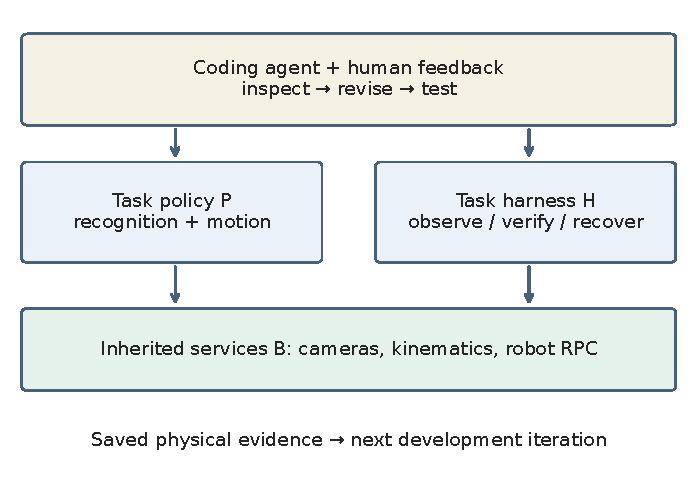
\includegraphics[width=\columnwidth]{harness_layers.pdf}
\caption{The mutable artifact has two layers: task policy and task harness.
Existing hardware services are inputs, not claimed inventions. Human feedback
guides development; the generated runtime executes without LLM servo calls.}
\label{fig:layers}
\end{figure}

Our two cases expose complementary supervision regimes. The door program
mines twelve successful archived teleoperation episodes and reuses a relative
pull trajectory. The cap program receives no cap-specific action demonstration
and instead uses a target click, local physical calibration, and observed
failures. Both must distinguish a grasp from a useful access-state transition:
the door must be open, or the cap must leave the bottle while remaining held.

The contributions are: (1) an explicit separation of editable policy,
editable task harness, and inherited hardware services; (2) a source- and
observation-grounded account of how physical failures changed these layers;
and (3) two executable laboratory manipulation case studies with separate
contact and object-state evidence. The experiments support feasibility and
mechanistic insight. They do not estimate a general success rate or establish
that harness adaptation is causally superior to a fixed-harness baseline.

\section{Related Work and Positioning}
Laboratory robot systems can support autonomous experimental searches, as
demonstrated by a mobile robotic chemist~\cite{chemist}. Here we study how the
required manipulation software is developed, rather than how experiments are
selected once that software is reliable.

\subsection{From generated policies to physical autoresearch}
Code as Policies uses language models to generate programs that compose robot
capabilities~\cite{cap}. VoxPoser grounds language-guided manipulation in
spatial representations and model-based planning~\cite{voxposer}. ReAct
illustrates iterative reasoning with action feedback~\cite{react}. These
approaches motivate executable programs as the interface between language
reasoning and a physical system. Our emphasis is the persistence and revision
of the machinery that makes a trial informative.

ENPIRE is the closest framework-level comparison~\cite{enpire}. Coding agents
first construct environment APIs with human feedback, then improve policies
through fixed reset and verification interfaces. ENPIRE supports demonstration
use, heuristic programs, gradient-based training, and hybrids with VLAs. The
distinction studied here is not ``manual versus automatic harness creation.''
It is the interleaving of harness revisions with policy development in a
laboratory deployment. Our case studies are smaller and are not a matched
performance or resource comparison with ENPIRE.

\subsection{Policy learning and external capabilities}
OpenVLA and $\pi_{0.5}$ learn broad motor behavior from large-scale data
~\cite{openvla,pi05}. A coding agent can complement such policies by changing
the observation representation, selecting a controller, or adding an outcome
test. Neither reported runtime used a task-specific VLA policy. This does not
establish that a VLA could not solve the tasks without new demonstrations.

External facilities also provide strong priors. SAM offers general-purpose
segmentation~\cite{sam}; MuJoCo provides model-based analysis~\cite{mujoco}.
The inherited stack included camera calibration, kinematics, and tested
teleoperation interfaces. We account for these resources explicitly rather
than attributing their capabilities to code generation from scratch. A useful
revision may remove a heavyweight dependency: both accepted task paths used
classical vision and depth rather than calling SAM in their critical runtime.

\section{RoboEvolve: The Development Artifact}
\subsection{Three layers with different responsibilities}
Let $B$ denote inherited robot services, $P$ the task policy, and $H$ the task
harness. A policy consumes observations and proposes motion. The harness
provides observation acquisition $O$, execution and interruption $X$, outcome
verification $V$, recovery $R$, and logging $L$:
\begin{equation}
 C=(P,H;B),\qquad H=(O,X,V,R,L).
\label{eq:artifact}
\end{equation}
This partition describes responsibilities, not a requirement that they be
separate packages. Target detection and local servoing belong to $P$; making
a fresh camera capture parseable belongs to $O$. A target aperture belongs to
motion; deciding whether the observed aperture permits another stage belongs
to $X$ or $V$. Driver gain setting remains an existing capability in $B$.

\begin{table}[t]\centering\small
\caption{Resource boundary in the reported deployment.}
\label{tab:boundary}
\begin{tabularx}{\columnwidth}{lY}\toprule
Category & Supplied or acquired resource\\\midrule
Inherited & Piper RPC/CAN and gripper interfaces; camera services; robot model and kinematics; prior repository context\\
Task supervision & Language goals and corrections; archived door episodes; one cap target click\\
External tools & OpenCV, NumPy, Record3D depth, fiducial registration, MuJoCo/Mink, Python subprocesses, tests and Git\\
Agent revisions & Contact frames, local visual models, task state machines, evidence checks, recovery and process handling\\
Physical evidence & Images, depth, measured pose/aperture, execution records and observed endpoints\\\bottomrule
\end{tabularx}
\end{table}

The agent does not have privileged physical truth. It learns about the cell
through the supplied services, files, and conversation. Existing scene models
may be wrong, and stored camera registration is valid only for its enrolled
configuration. The observation record must therefore state which quantities
are measured and which are inferred.

\subsection{An evidence-driven revision loop}
A development iteration has five operations: acquire fresh observations;
execute a bounded stage; inspect discrepancies; revise a relevant component;
and test the revision. The agent can introduce numerical estimators and new
connections between existing tools. Human corrections may resolve instance
identity or geometry that the observations leave ambiguous. The development
trajectory can be written schematically as
\begin{equation}
 (P_{k+1},H_{k+1})=A(P_k,H_k,E_k,U_k;B),
\label{eq:update}
\end{equation}
where $A$ is the coding-agent process, $E_k$ physical evidence, and $U_k$
operator input. This equation is a description, not an implemented optimizer
with a fixed differentiable objective. In the historical trials, success
criteria themselves were refined as failures exposed inadequate evidence.

For that reason, revisions and evidence must not be conflated. Saved images
and robot states remain the reference record. If an evaluator changes, its
version and rationale must be distinguished from a later retrospective
assessment. A program becoming easier to satisfy is not proof of improved
robot behavior. Our retrospective analysis uses common saved measurements and
endpoint evidence where available, and leaves missing outcomes unclassified.

\subsection{Promotion to a deterministic runtime}
The accepted program is a stage machine with measured preconditions and
outcome checks. The language model is involved in constructing and revising
the program, not in producing every control command. Motion uses the existing
robot command path, with short-lived observation tools and structured results.
Task-specific tests and versioned code preserve the behavior beyond the
conversation that produced it.

Promotion can be partial. If closure, lift, and transport are supported but
placement is not, the program's reported capability ends at held transport.
This prevents a successful prefix from being either discarded wholesale or
overstated as a completed longer workflow. Hardware evidence for one route
also does not authorize arbitrary new routes: a simulator discrepancy was
scoped to an exact, hashed cap waypoint sequence rather than generalized into
a blanket collision exception.

\subsection{Implementation substrate}
\begin{table}[t]\centering\small
\caption{Schematic execution contract, assembled from the accepted stage
logic. It describes runtime decisions, not autonomous code generation.}
\label{tab:contract}
\begin{tabularx}{\columnwidth}{lY}\toprule
Stage & Required evidence or decision\\\midrule
Observe & Acquire current target and robot observations; reject missing evidence\\
Align & Apply task-specific visual/geometric correction before contact\\
Engage & Close once and establish a non-empty grasp\\
Move & Execute a checked segment; test retention at the available checkpoints\\
Inspect & Door: classify endpoint independently. Cap: confirm removal relative to support\\
Recover & Stop on missing grasp; use scoped recovery rather than repeating blindly\\
Promote & Preserve the verified prefix and its inputs; leave unsupported suffixes unclaimed\\\bottomrule
\end{tabularx}
\end{table}

The physical system comprises two Piper arms, RGB wrist cameras, and a fixed
Record3D RGB-D camera. The reported actions use the right arm and measured
gripper opening. NumPy supports numerical fitting; OpenCV supports image
components and registration; Mink/MuJoCo support kinematics and model-based
checks. The trajectory adapter sends end-effector targets through the same
robot interface used by teleoperation. Acquisition and analysis run outside
the servo loop. No new robot driver or foundation perception model was trained.

The final critical paths are intentionally heterogeneous. Door control uses a
demonstration compiler, a plane estimator, visual offsets, and a grasp checker.
Cap control uses relational appearance, local calibration, and support-aware
verification. The fact that both can be assembled with one coding-agent
workflow does not make their perception interchangeable.

\section{Case I: Opening and Closing an Incubator}
\subsection{Supervision becomes a reusable representation}
The operator introduced an existing door archive and its location before it
was used. Of 57 candidate teleoperation episodes, twelve terminal images were
verified as successful openings and admitted to compilation. These are twelve
trajectories, not twelve isolated state samples. One actual medoid episode
provided the relative pull, with the contact frame factored out:
\begin{equation}
 T_k=T_c^{\rm live}(T_c^{\rm demo})^{-1}T_k^{\rm demo}.
\end{equation}
This retained a demonstrated articulated motion while allowing current
contact alignment. The same data also informed local visual correction.

The first important correction was representational. The initial live pose
was not the correct contact anchor. Starting instead from demonstrated
pre-close geometry removed a large approach discrepancy. Head-depth plane
fitting then estimated appliance yaw, and bounded wrist-image correction
adjusted lateral contact. A dark feature previously treated as meaningful was
identified by the operator as a shadow and excluded.

\subsection{A policy failure exposes a harness failure}
The first structured pull retained opening after a 5\,mm proof but lost
contact during the longer motion. The initial implementation could complete
the remaining trajectory without verifying retention along the way. The
revision slowed the pull to twice the demonstration duration, inserted checks
every 15 frames at a 30\,Hz command rate, and added stop/retreat/open recovery.
This changed both the motion schedule and the execution harness.

Further trials still slipped, showing that the new harness detected failure
but did not alone solve manipulation. Depth-based yaw alignment and fresh
contact anchoring preceded the later open endpoints. The accepted controller
closed once, required stable non-empty opening, performed the 5\,mm proof,
and reverified retention while stationary before the long pull.

Most importantly, loss of contact did not determine the task outcome. T1 and
T2 were closed at their evaluated endpoints; T6 and T7 were open. All four
had opening near 0.0034 afterward. Thus an aperture-only evaluator would
conflate distinct physical outcomes. Registered head-depth comparison against
open and closed references became a separate evaluator.

\begin{figure*}[t]\centering
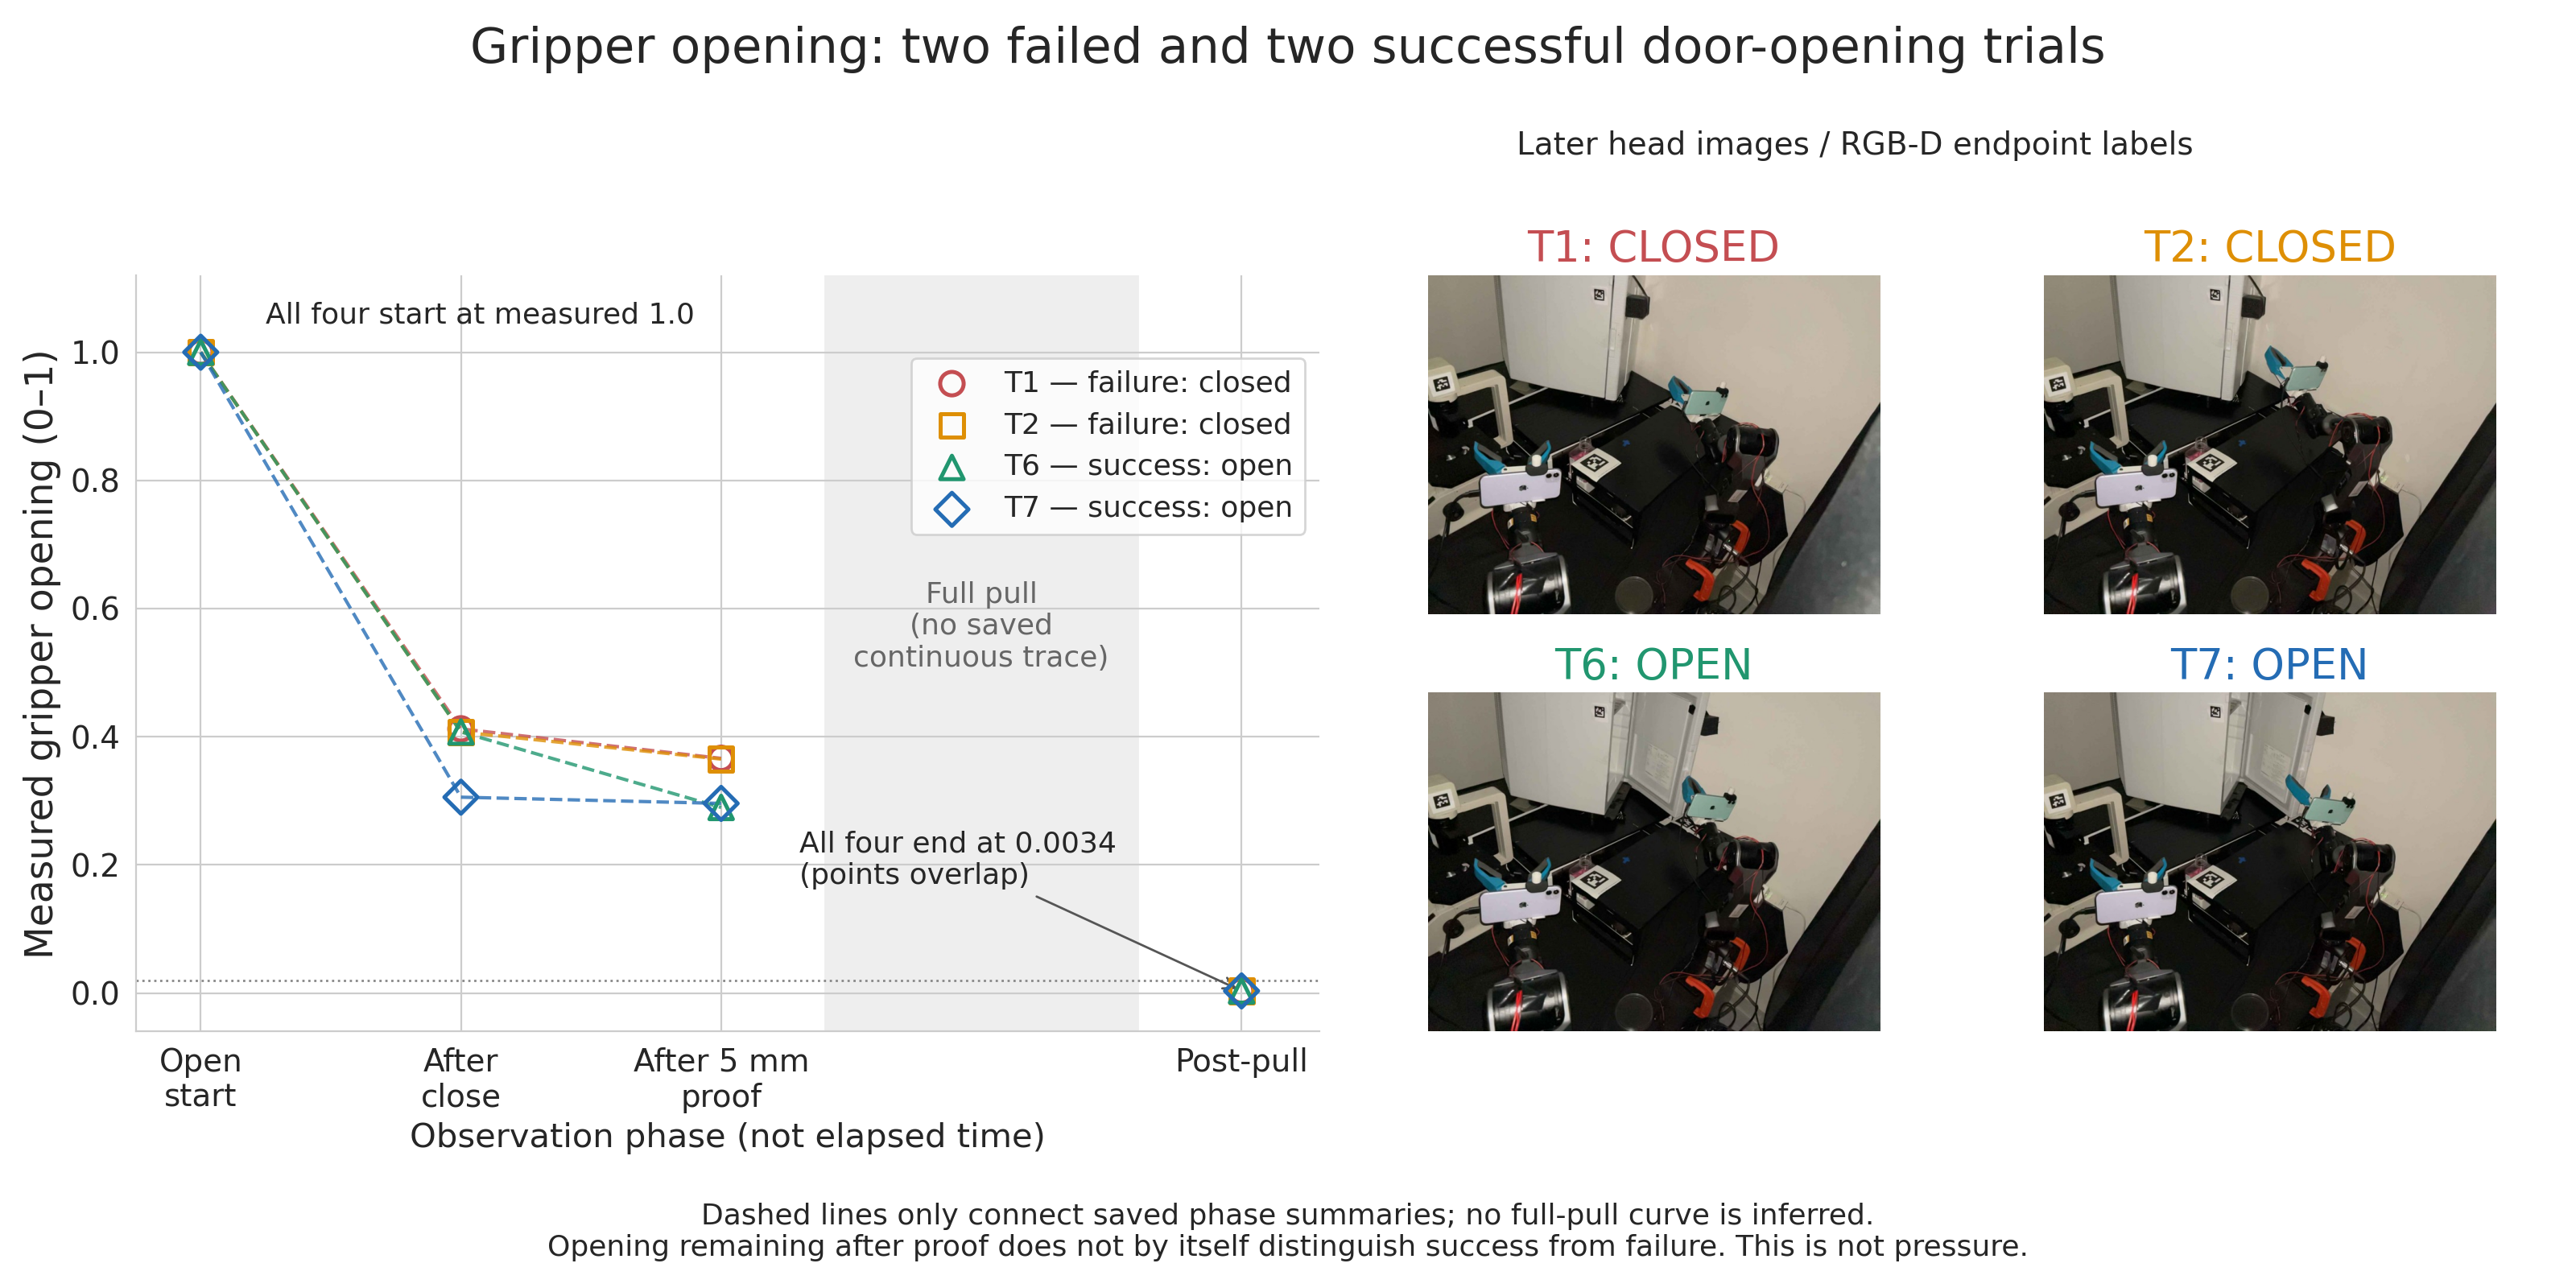
\includegraphics[width=.92\textwidth]{door_grasp_outcome_overlay.png}
\caption{Why a task harness needs independent outcome evidence. T1/T2 end
closed; T6/T7 end open, although each later aperture is approximately 0.0034.
The dots are saved phase observations or summaries, not a full time trace.
The blank full-pull region marks unavailable continuous measurements. Right:
later head views associated with the respective trials.}
\label{fig:outcomes}
\end{figure*}

\subsection{Observation and evaluation also required repair}
One autonomous launch failed because native camera messages were mixed with
JSON output. Parsing the structured result robustly allowed orchestration to
proceed; it did not change the underlying door trajectory. Arm contamination
of a depth mask led to an evaluator correction. These changes are neither
new action-network weights nor new physical skills, but they are necessary
for a usable development and execution loop.

The final recorded autonomous opening began from a classified closed state,
performed one approximately 3.5\,mm visual correction, passed proof and
stationary checks, and stopped when later opening indicated an empty grasp.
The subsequent registered endpoint was open. The evidence supports opening
with later grasp loss, without resolving the precise opening/slip chronology.

Closing required a different task policy. Reversing the opening path missed
the useful pushing location by about 15\,cm in height. A dedicated closing
demonstration supplied the accepted open-jaw push; a separate autonomous run
verified a closed endpoint. The twelve opening demonstrations should therefore
not be reported as the total supervision for both directions.

\section{Case II: Removing and Retaining a Bottle Cap}
\subsection{No action demonstration; local identification instead}
The cap case did not receive a task-specific teleoperation trajectory. It did
receive one target click, language corrections, and access to the existing
robot stack. A detector based on global whiteness initially selected unrelated
components. The revised representation used the relation ``cap above this
colored bottle neck'' and anchored the instance to the click. Jaw geometry
defined the relevant image error, rather than a generic image-center target.

Seven open-jaw observations supported a local image Jacobian. For image error
$e$ and robot displacement $\Delta x$, the controller approximated
$\Delta e=J\Delta x$ and applied bounded corrections from $-J^+e$. This is
task-local system identification, not a claim that seven samples train a
general robot policy. Lateral alignment preceded descent because the bottle
was recessed between platforms; the incorrect support model had previously
misled the approach.

Registered depth updated the selected surface and completed bottle/cap
geometry. MuJoCo/Mink checked candidate paths, while hardware observations
retained authority over the one exact route whose model prediction disagreed
with measured execution. The final target detector used OpenCV operations.
An import from a module with ``SAM'' in its name supplied color constants,
not a SAM inference call. This source-level distinction matters when counting
which external tools actually contributed to the accepted controller.

\subsection{Verification is a sequence of distinct contracts}
The cap harness separates four statements: the jaws engage the cap; the cap
leaves the bottle; the cap remains held during transport; and the cap is
placed stably. Each requires a different witness. A retained aperture can
support grasping but cannot alone establish source clearance. A rising robot
pose cannot exclude lifting the entire bottle. An open gripper at a destination
cannot prove that the cap rests there.

The accepted closure check required the target within the jaw segment, a
perpendicular offset no greater than 0.25 jaw spans, non-empty opening between
0.10 and 0.40, and limited bottle motion. Lift added at least 8\,mm of measured
vertical rise, source-appearance reduction, and retained opening. Transport
added at least 50\,mm displacement, limited aperture drift, and continued
support stability. The thresholds define the accepted local audit; they are
not universal physical constants or evidence of calibrated force sensing.

\begin{figure*}[t]\centering
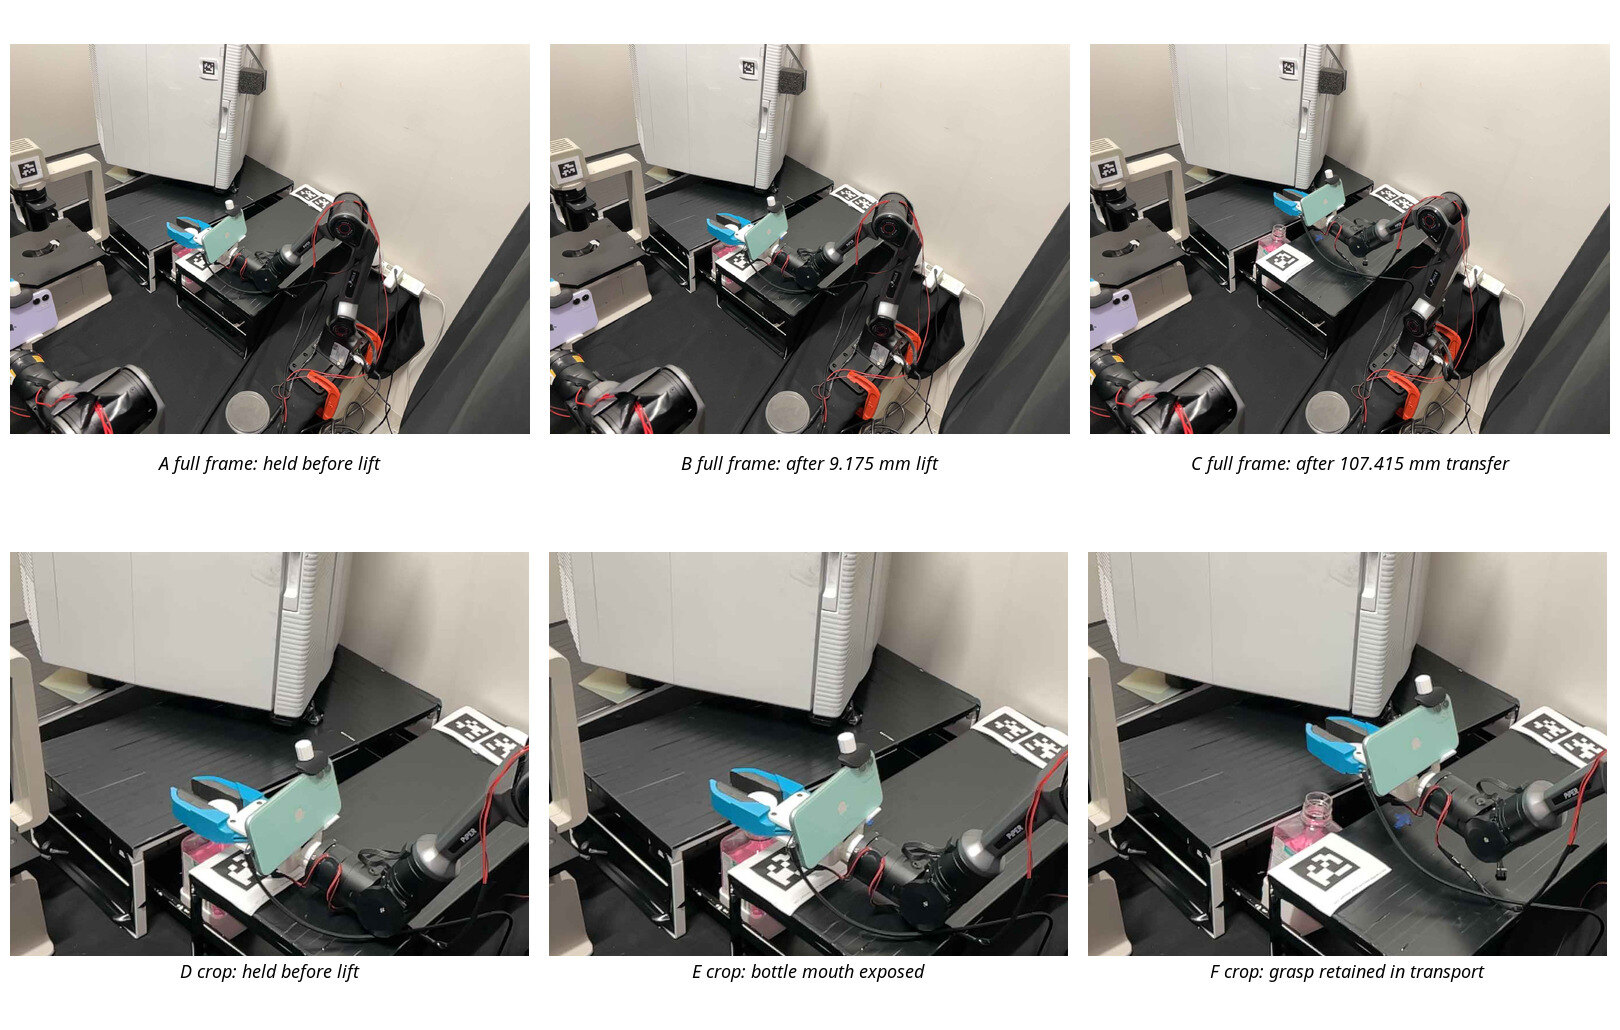
\includegraphics[width=.90\textwidth]{cap_verified_transfer_rgb.jpg}
\caption{Cap evidence used for staged verification. The same capture triplet
supports pre-lift engagement, 9.17\,mm measured rise, and 107.42\,mm subsequent
held transport. Full views and detail crops expose both the target and bottle
support. These are stages of one sequence, not independent success repetitions.}
\label{fig:cap}
\end{figure*}

\subsection{Measured capability and deliberately excluded suffix}
The pre-lift, post-lift, and post-transport openings were 0.20057, 0.20143,
and 0.20114. End-effector height increased by 9.17\,mm during lift, and
subsequent displacement was 107.42\,mm. The source's cap-like appearance
fraction fell from 0.4482 to 0.1684 after lift and stayed at 0.1698 after
transport. Bottle-support shift after lift was 0.0095 of its visual scale.
These complementary observations support removal and retained transport.

A later release was not promoted to verified placement because destination
support evidence was insufficient. The accepted program therefore preserves
the successful prefix. No threaded unscrewing, torque-controlled loosening,
resealing, or aseptic outcome was demonstrated. The capability is useful but
specific: side-pinch removal and held transport of the observed cap.

\section{Cross-Case Analysis}
\subsection{What changed beyond the policy?}
Table~\ref{tab:changes} classifies representative revisions by responsibility.
The classification is intentionally conservative: adding a visual servo is a
policy change, not automatically a new harness. In contrast, repairing camera
output handling or changing which evidence is required to declare an endpoint
does alter the task harness.

\begin{table*}[t]\centering\small
\caption{Physical evidence and the resulting program revision. These are
historically associated changes, not isolated causal ablations.}
\label{tab:changes}
\begin{tabularx}{\textwidth}{p{.24\textwidth}YY}\toprule
Observed problem & Policy revision & Harness revision\\\midrule
Initial pose was not handle contact & Demonstrated contact-relative anchor & Explicit contact-reference checks\\
Proof passed; long pull lost grasp & Slower full-pull schedule & Periodic retention checks and recovery\\
Empty jaws after different door outcomes & No automatic repetition of the pull & Registered open/closed endpoint inspection\\
Camera diagnostics mixed with JSON & No motion change required & Structured output extraction / process handling\\
Arm entered the door-state mask & No motion change required & Restrict endpoint evidence region\\
White distractor mistaken for cap & Click-anchored cap/neck relation & Preserve target identity through stages\\
Bottle recessed between platforms & Correct support model and approach order & Model/hardware disagreement audit\\
Lift or release did not prove completion & Preserve verified egress route & Separate removal, retention, placement checks\\\bottomrule
\end{tabularx}
\end{table*}

The strongest example is the door endpoint. A policy that loses the handle
after opening has a different task outcome from a policy that loses it before
opening, yet their final aperture observations can be equal. A better policy
alone does not make an aperture-only evaluator informative. The interface
must expose evidence about the door. For the cap, the analogous additional
variable is the supporting bottle: target motion must be distinguished from
support motion.

This does not establish that a coding agent is uniquely able to discover
these checks. A human engineer could design them. The empirical contribution
is that the recorded coding-agent workflow implemented them while revising
the controller, and left executable artifacts and tests rather than relying
only on conversational instructions at deployment time.

\subsection{Quantitative diagnostics and their interpretation}
We show all ten preserved door contact poses in Fig.~\ref{fig:orientation}.
The full rotation difference to T7 is computed from normalized quaternions as
$2\arccos(\min(1,|q_i^\top q_7|))$. T1--T5 differ by approximately
$8.9$--$9.5^\circ$, while T6 differs by $2.39^\circ$. This is consistent with
the late orientation revisions. T7 is a retrospectively chosen reference;
its zero error is definitional and does not measure task optimality. The
diagnostic does not compensate for door pose changes or prove that orientation
alone caused opening.

\begin{figure}[t]\centering
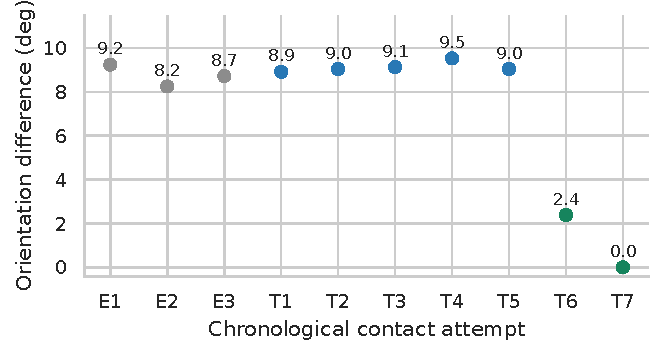
\includegraphics[width=\columnwidth]{orientation.pdf}
\caption{A policy-level diagnostic within the broader development history.
All preserved contact orientations are compared with T7, not with an unseen
ground-truth optimum. Colors distinguish early contacts, T1--T5, and the two
open endpoints.}
\label{fig:orientation}
\end{figure}

The opening result consists of an observed yaw-aligned open endpoint and one
verified autonomous open endpoint, with a separate verified close run. The cap
result is one audited removal/transport sequence. Trials were developmental,
not identically reset independent draws. Neither endpoint counts nor code
revision counts are treated as a population success rate. A larger tool graph
also does not imply a better controller: the accepted paths excluded SAM
inference and task-specific neural-policy training despite their availability.

\subsection{Reproducibility does not mean a complete trace}
Source snapshots, selected tool records, and saved images/state can establish
which program ran and what was observed. They cannot recover measurements
that were never persisted. Some full-pull aperture checks were accumulated
in memory and lost on exceptions before serialization. The later audit found
slip-stop messages but not the missing continuous trace. Sparse joint-torque
warnings also do not measure contact pressure or a break-away force curve.

We therefore preserve missingness in plots and tables. Cap displacement is
computed from robot state and corroborated by images, not reported as a
submillimeter object-tracking accuracy. Historical evaluator repairs are
distinguished from retrospective scoring. This is important when the learner
can edit the evaluator: the archive must support checking the physical claim
independently of the code's own success flag.

\section{Discussion}
\subsection{Why laboratory constraint release is a useful test}
Door opening and cap removal require access-state changes under clutter and
partial occlusion. Unlike a motion-only objective, each has a supporting body
that should remain appropriately constrained: the hinge for the door, and the
bottle for the cap. Contact can disappear because a useful release occurred
or because the grasp failed. Explicit world-state verification resolves an
ambiguity that would otherwise contaminate the development signal.

The two tasks should not be called harder than insertion or cutting without
a matched evaluation. Nor do they establish force-controlled break-away
behavior. Their value here is exposing different failure modes to a shared
code-development process. They are prerequisites for laboratory workflows,
not demonstrations of an automated biological discovery pipeline. Sample
integrity, contamination control, and biological outcomes remain outside the
reported evaluation.

\subsection{Adaptable infrastructure needs a stable reference}
Allowing $V$ to change creates a risk: a weaker test can make the same behavior
look better. The reported history contains evaluator refinement rather than a
pre-registered immutable scoring protocol. Our safeguard in this analysis is
to retain observations, identify revisions, and restrict claims to externally
inspectable endpoints. This retrospective discipline is not equivalent to a
prospective anti-reward-hacking guarantee.

A direct future test would initialize identical repositories and allocate
equal trial and human-feedback budgets to fixed-$H$ and editable-$H$
conditions. An external evaluator, held fixed in both, would measure success,
false-positive completion, time to a verified result, and intervention count.
This would test whether co-evolution improves capability rather than merely
changing its definition. No such ablation is presented as completed here.

\subsection{The role of accumulated context}
The coding agent had access to prior repository work and conversation, not
just a minimal task prompt. Some infrastructure and lessons were inherited.
This is a realistic laboratory collaborator setting, but it prevents a claim
of learning from scratch. Task demonstrations, operator corrections, existing
tools, and agent-written code must be accounted for separately.

The reusable outcome is also more limited than universal transfer. Contact
frames, support witnesses, stage checks, and process adapters can be reused,
while appearance thresholds, registration, and routes require revalidation
when the environment changes. A clean-start replication with a declared
resource manifest is the natural next step. The present evidence shows how
capability emerged, not how often an independently initialized agent will
rediscover it.

\section{Conclusion}
\system\ treats physical feedback as a reason to revise the task harness as
well as the robot policy. In laboratory door and cap manipulation, failures
changed contact representations, visual models, execution checks, observation
handling, and outcome verification. The resulting programs achieved recorded
access-state transitions and ran without an LLM in the servo loop. The
central lesson is that improving robot behavior and improving the machinery
that observes and validates that behavior are coupled engineering problems.
An auditable coding-agent workflow makes that coupling explicit and testable.

\section*{Acknowledgments and AI Use Disclosure}
OpenAI Codex assisted with manuscript drafting, analysis scripts, and figure
layout throughout this article. Codex also generated and revised experimental
robot code as the system under study. Experimental photographs are recorded
camera images, not generative images. This disclosure distinguishes manuscript
assistance from the robot-development intervention evaluated here.

\bibliographystyle{IEEEtran}
\bibliography{references}
\end{document}
